%*****************************************
\chapter{Mathematical Computations}\label{ch02:mathematical_computations}
%*****************************************

\chapter{Mathematical Computations}

Perhaps the most valuable feature of Excel is its ability to produce mathematical outputs using the data in a workbook. This chapter reviews several mathematical outputs that you can produce in Excel through the construction of formulas and functions. The chapter begins with the construction of formulas for basic and complex mathematical computations. The second section reviews statistical functions, such as SUM, AVERAGE, MIN, and MAX, which can be applied to a range of cells. The last section of the chapter addresses functions used to calculate mortgage and lease payments as well as the valuation of investments. This chapter also shows how you can use data from multiple worksheets to construct formulas and functions. These skills will be demonstrated in the context of a personal cash budget, which is a vital tool for managing your money for long-term financial security. The personal budget objective will also provide you with several opportunities to demonstrate Excel's what-if scenario capabilities, which highlight how formulas and functions automatically produce new outputs when one or more inputs are changed.

\section{Formulas}

\begin{center}
	\begin{objbox}{Learning Objectives}
		\begin{itemize}
			\setlength{\itemsep}{0pt}
			\setlength{\parskip}{0pt}
			\setlength{\parsep}{0pt}
			
			\item Learn how to create basic formulas.
			\item Understand relative referencing when copying and pasting formulas.
			\item Work with complex formulas by controlling the order of mathematical operations.
			\item Understand formula auditing tools.

		\end{itemize}
	\end{objbox}
\end{center}

This section reviews the fundamental skills for entering formulas into an Excel worksheet. The objective used for this chapter is the construction of a personal cash budget. Most financial advisors recommend that all households construct and maintain a personal budget to achieve and maintain strong financial health. Organizing and maintaining a personal budget is a skill you can practice at any point in your life. Whether you are managing your expenses during college or maintaining the finances of a family of four, a personal budget can be a vital tool when making financial decisions. Excel can make managing your money a fun and rewarding exercise.

Figure \ref{02:fig01} shows the completed workbook that will be demonstrated in this chapter. Notice that this workbook contains four worksheets. The first worksheet, \textbf{Budget Summary}, contains formulas that utilize or reference the data in the other three worksheets. As a result, the \textbf{Budget Summary} worksheet serves as an overview of the data that was entered and calculated in the other three worksheets of the workbook.

\begin{figure}[H]
	\centering
	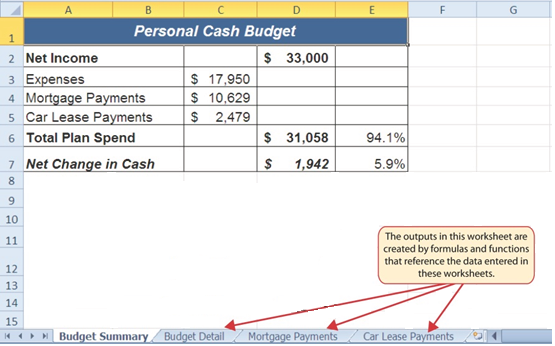
\includegraphics[width=\maxwidth{.95\linewidth}]{gfx/ch02_fig01}
	\caption{Completed Personal Budget Workbook}
	\label{02:fig01}
\end{figure}

\subsection{Creating a Basic Formula}

\textit{Download Data File: CH2 Data}

Formulas are used to calculate a variety of mathematical outputs in Excel and can be used to create virtually any custom calculation required for your objective. Furthermore, when constructing a formula in Excel, you use cell locations that, when added to a formula, become cell references. This means that Excel uses, or references, the number entered into the cell location when calculating a mathematical output. As a result, when the numbers in the cell references are changed, Excel automatically produces a new output. This is what gives Excel the ability to create a variety of what-if scenarios, which will be explained later in the chapter.

To demonstrate the construction of a basic formula, we will begin working on the \textbf{Budget Detail} worksheet in the Personal Budget workbook, which is shown in Figure \ref{02:fig02}. To complete this worksheet, we will add several formulas and functions. Table \ref{02:tab01} provides definitions for each of the spend categories listed in the range \textsf{A3:A11}. When you develop a personal budget, these categories are defined on the basis of how you spend your money. It is likely that every person could have different categories or define the same categories differently. Therefore, it is important to review the definitions in Table \ref{02:tab01} to understand how we are defining these categories before proceeding.

\begin{figure}[H]
	\centering
	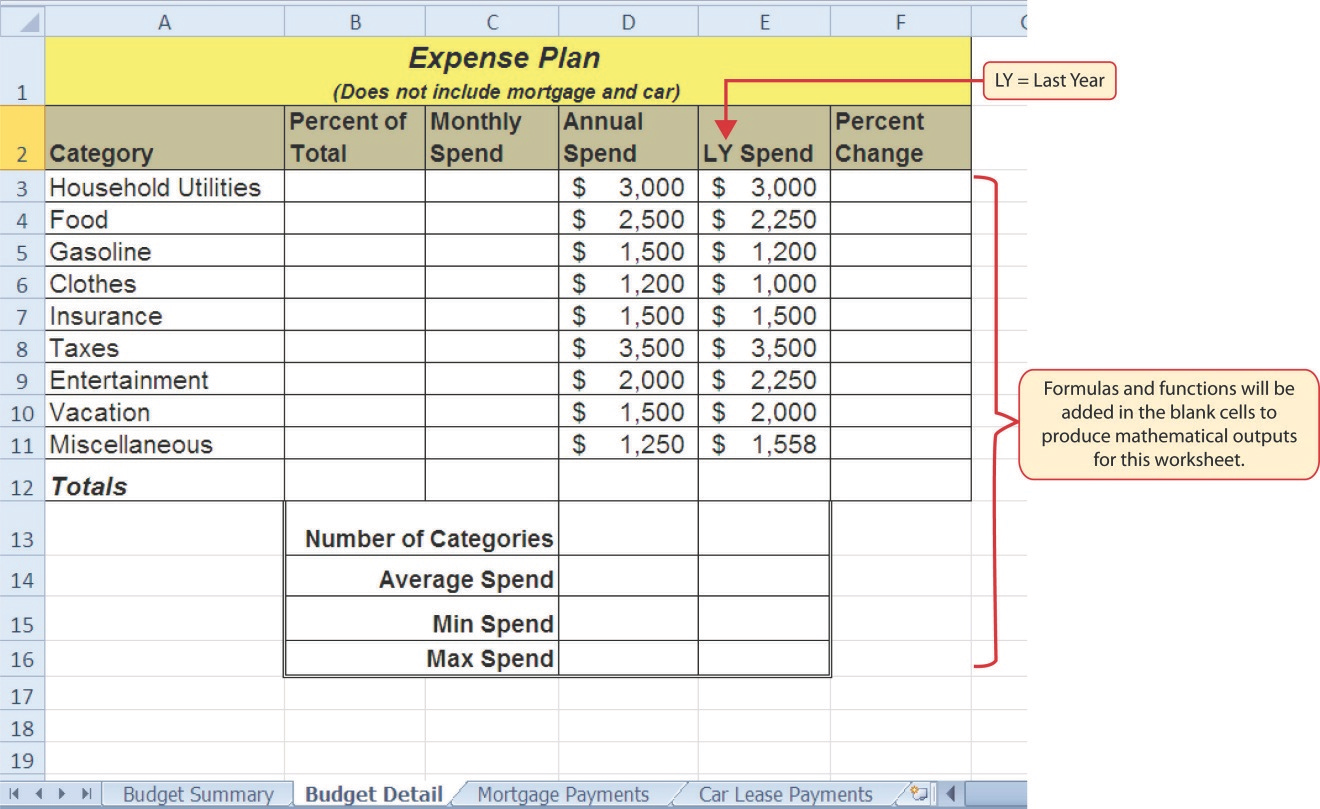
\includegraphics[width=\maxwidth{.95\linewidth}]{gfx/ch02_fig02}
	\caption{Budget Detail Worksheet}
	\label{02:fig02}
\end{figure}

{\small
	\begin{longtable}{p{0.85in}p{2.8in}}
		\textbf{Category} & \textbf{Definition} \endhead
		\hline \\
		Household\newline Utilities & Money spent on electricity, heat, and water and on cable, phone, and Internet access\\
		Food & Money spent on groceries, toiletries, and related items\\
		Gasoline & Money spent on fuel for automobiles\\
		Clothes & Money spent on clothes, shoes, and accessories\\
		Insurance & Money spent on homeowner's or automobile insurance\\
		Taxes & Money spent on school and property taxes (this example of the personal budget assumes that we own property)\\
		Entertainment & Money spent on entertainment, including dining out, movie and theater tickets, parties, and so on\\
		Vacation & Money spent on vacations\\
		Miscellaneous & Includes any other spending categories, such as textbooks, software, journals, school or work supplies, and so on\\
		\hline
		\caption{Spend Category Definitions}
		\label{02:tab01}
	\end{longtable}
}

The first formula that we will add to the \textbf{Budget Detail} worksheet will calculate the Monthly Spend values. The formula will be constructed so that it takes the values in the Annual Spend column and divides them by $ 12 $. This will show how much money will be spent per month for each of the categories listed in Column \textsf{A}. The following explains how this formula is created.

\begin{enumerate}
	\item Open the Data file named \textbf{CH2 Data} and use the File/Save As command to save it with the new name \textbf{CH2 Personal Budget}.
	\item Click the \textbf{Budget Detail} worksheet tab to open the worksheet.
	\item Click cell \textsf{C3}.
	\item Type an equal sign $ = $. When the first character entered into a cell location is an equal sign, it signals Excel to perform a calculation or produce a logical output.
	\item Type \textsf{D3}. This adds \textsf{D3} to the formula, which is now a cell reference. Excel will use whatever value is entered into cell \textsf{D3} to produce an output.
	\item Type the slash symbol $ / $. This is the symbol for division in Excel. As shown in Table \ref{02:tab02} the mathematical operators in Excel are slightly different from those found on a typical calculator.
	\item Type the number $ 12 $. This divides the value in cell \textsf{D3} by $ 12 $. In this formula, a number, or constant, is used instead of a cell reference because it will not change. In other words, there will always be $ 12 $ months in a year.
	\item Press the ENTER key.
\end{enumerate}

\begin{longtable}{p{0.85in}p{2.8in}}
	\textbf{Symbol} & \textbf{Operation} \endhead
	\hline \\
	$ + $ & Addition\\
	$ - $ & Subtraction\\
	$ / $ & Division\\
	$ * $ & Multiplication\\
	$ \wedge $ & Power/Exponent\\
	\hline
	\caption{Excel Mathematical Operators}
	\label{02:tab02}
\end{longtable}


Figure \ref{02:fig03} shows how the formula appears in cell \textsf{C3} before you press the ENTER key. Figure \ref{02:fig04} shows the output of the formula after you press the ENTER key. The Monthly Spend for Household Utilities is \$250 because the formula is taking the Annual Spend in cell \textsf{D3} and dividing it by 12. If the value in cell \textsf{D3} is changed, the formula automatically produces a new output. We are calculating the spend per month for each category because people often get paid and are billed for these items on a monthly basis. This formula allows you to compare your monthly income to your monthly bills to determine whether you have enough income to pay these expenses.

\begin{figure}[H]
	\centering
	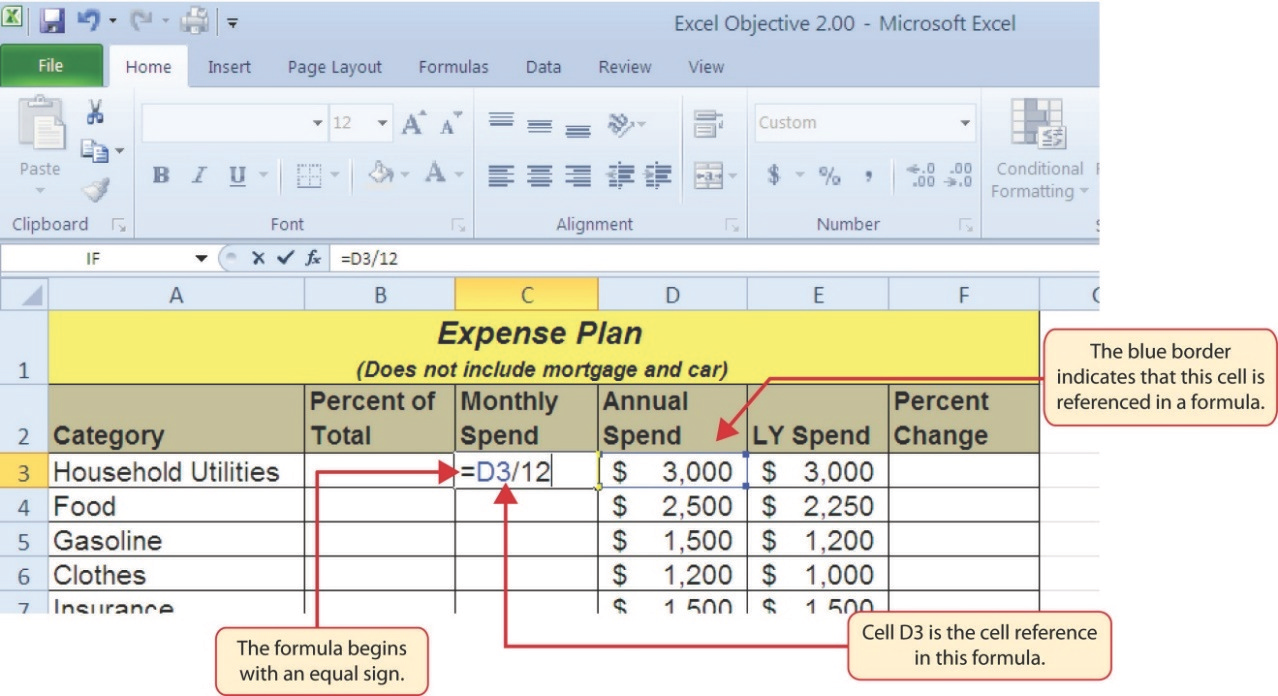
\includegraphics[width=\maxwidth{.95\linewidth}]{gfx/ch02_fig03}
	\caption{Adding a Formula to a Worksheet}
	\label{02:fig03}
\end{figure}

\begin{figure}[H]
	\centering
	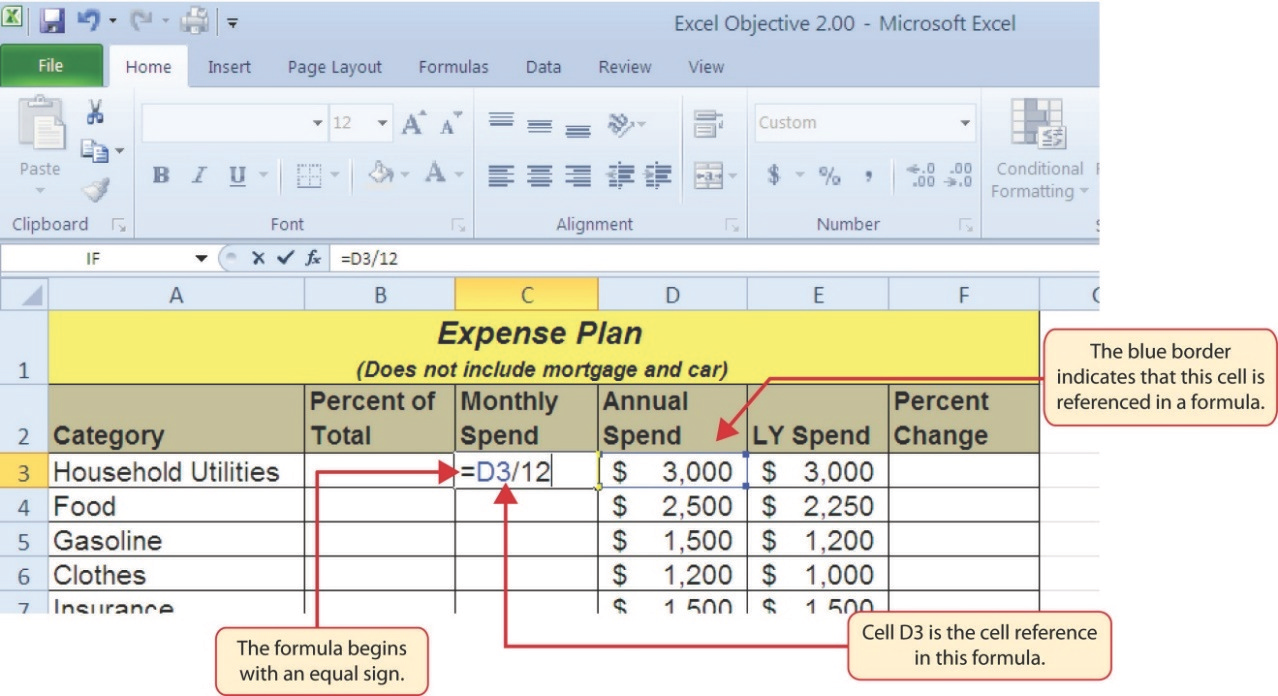
\includegraphics[width=\maxwidth{.95\linewidth}]{gfx/ch02_fig04}
	\caption{Formula Output for Monthly Spend}
	\label{02:fig04}
\end{figure}

\begin{center}
	\begin{infobox}{Why?}
		\textbf{Use Cell References}
		\\
		\\
		Cell references enable Excel to dynamically produce new outputs when one or more inputs in the referenced cells are changed. Cell references also allow you to trace how outputs are being calculated in a formula. As a result, you should never use a calculator to determine a mathematical output and type it into the cell location of a worksheet. Doing so eliminates Excel's cell-referencing benefits as well as your ability to trace a formula to determine how outputs are being produced.
	\end{infobox}
\end{center}

\subsection{Relative References (Copying and Pasting Formulas)}

Once a formula is typed into a worksheet, it can be copied and pasted to other cell locations. For example, Figure \ref{02:fig04} shows the output of the formula that was entered into cell \textsf{C3}. However, this calculation needs to be performed for the rest of the cell locations in Column \textsf{C}. Since we used the \textsf{D3} cell reference in the formula, Excel automatically adjusts that cell reference when the formula is copied and pasted into the rest of the cell locations in the column. This is called relative referencing and is demonstrated as follows.

\begin{enumerate}
	\item Click cell \textsf{C3}.
	\item Place the mouse pointer over the Auto Fill Handle.
	\item When the mouse pointer turns from a white block plus sign to a black plus sign, click and drag down to cell \textsf{C11}. This pastes the formula into the range \textsf{C4:C11}.
	\item Double click cell \textsf{C6}. Notice that the cell reference in the formula is automatically changed to \textsf{D6}.
	\item Press the ENTER key.
\end{enumerate}

Figure \ref{02:fig05} shows the outputs added to the rest of the cell locations in the Monthly Spend column. For each row, the formula takes the value in the Annual Spend column and divides it by 12. You will also see that cell \textsf{D6} has been double clicked to show the formula. Notice that Excel automatically changed the original cell reference of \textsf{D3} to \textsf{D6}. This is the result of relative referencing, which means Excel automatically adjusts a cell reference relative to its original location when it is pasted into new cell locations. In this example, the formula was pasted into eight cell locations below the original cell location. As a result, Excel increased the row number of the original cell reference by a value of one for each row it was pasted into.

\begin{figure}[H]
	\centering
	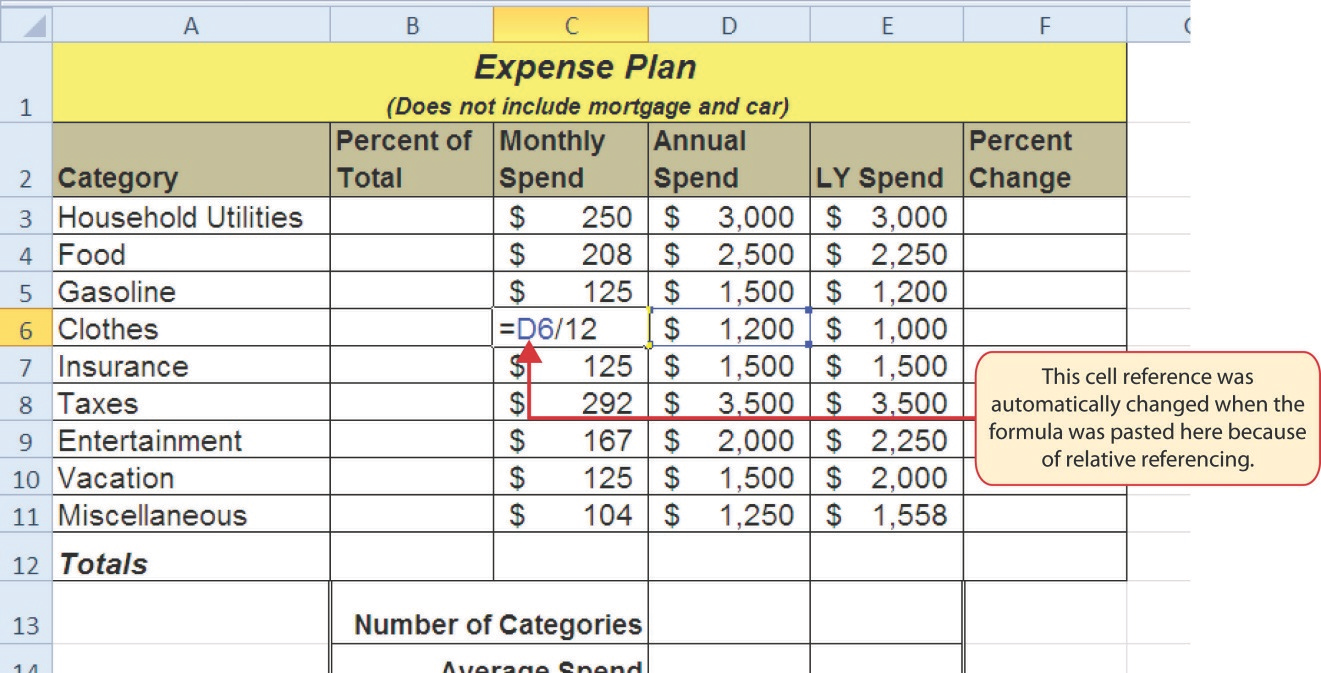
\includegraphics[width=\maxwidth{.95\linewidth}]{gfx/ch02_fig05}
	\caption{Relative Reference Example}
	\label{02:fig05}
\end{figure}

\begin{center}
	\begin{infobox}{Why?}
		\textbf{Use Universal Constants}
		\\
		\\
		If you are using constants, or numerical values, in an Excel formula, they should be universal constants that do not change, such as the number of days in a week, weeks in a year, and so on. Do not type the values that exist in cell locations into an Excel formula. This will eliminate Excel's cell-referencing benefits, which means if the value in the cell location you are using in a formula is changed, Excel will not be able to produce a new output.
	\end{infobox}
\end{center}

\subsection{Creating Complex Formulas (Controlling the Order of Operations)}

The next formula to be added to the Personal Budget workbook is the percent change over last year. This formula determines the difference between the values in the LY (Last Year) Spend column and shows the difference in terms of a percentage. This requires that the order of mathematical operations be controlled to get an accurate result. Table 2.3 shows the standard order of operations for a typical formula. To change the order of operations shown in the table, we use parentheses to process certain mathematical calculations first. This formula is added to the worksheet as follows.

\begin{enumerate}
	\item Click cell \textsf{F3} in the Budget Detail worksheet.
	\item Type an equal sign $ = $.
	\item Type an open parenthesis $ ( $.
	\item Click cell \textsf{D3}. This will add a cell reference to cell \textsf{D3} to the formula. When building formulas, you can click cell locations instead of typing them.
	\item Type a minus sign $ - $.
	\item Click cell \textsf{E3} to add this cell reference to the formula.
	\item Type a closing parenthesis $ ) $.
	\item Type the slash $ / $ symbol for division.
	\item Click cell \textsf{E3}. This completes the formula that will calculate the percent change of last year's actual spent dollars vs. this year's budgeted spend dollars (see Figure \ref{02:fig06}).
	\item Press the ENTER key.
	\item Click cell \textsf{F3} to activate it.
	\item Place the mouse pointer over the Auto Fill Handle.
	\item When the mouse pointer turns from a white block plus sign to a black plus sign, click and drag down to cell \textsf{F11}. This pastes the formula into the range \textsf{F4:F11}.
\end{enumerate}

\begin{figure}[H]
	\centering
	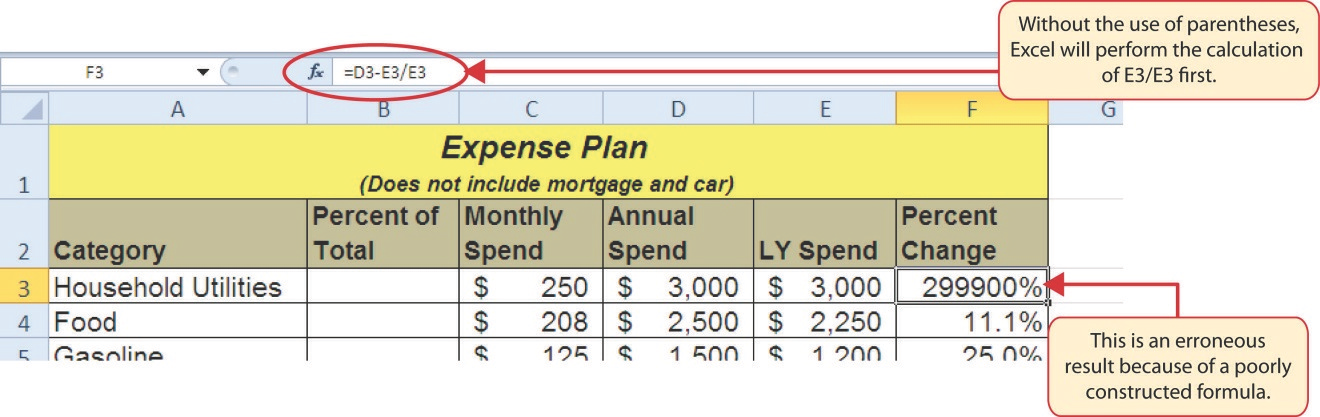
\includegraphics[width=\maxwidth{.95\linewidth}]{gfx/ch02_fig06}
	\caption{Adding the Percent Change Formula}
	\label{02:fig06}
\end{figure}

\begin{longtable}{p{0.85in}p{2.8in}}
	\textbf{Symbol} & \textbf{Operation} \endhead
	\hline \\
	$ () $ & Override Standard Order: Any mathematical computations placed in parentheses are performed first and override the standard order of operations. If there are layers of parentheses used in a formula, Excel computes the innermost parentheses first and the outermost parentheses last.\\
	$ \wedge $ & First: Excel executes any exponential computations first.\\
	$ * $ or $ / $ & Second: Excel performs any multiplication or division computations second. When there are multiple instances of these 	computations in a formula, they are executed in order from left to right.\\
	$ + $ or $ - $ & Third: Excel performs any addition or subtraction computations third. When there are multiple instances of these 	computations in a formula, they are executed in order from left to right.\\
	\hline
	\caption{Standard Order of Mathematical Operations}
	\label{02:tab03}
\end{longtable}

\begin{center}
	\begin{infobox}{Why?}
		\textbf{Use Relative Referencing}
		\\
		\\
		Relative referencing is a convenient feature in Excel. When you use cell references in a formula, Excel automatically adjusts the cell references when the formula is pasted into new cell locations. If this feature were not available, you would have to manually retype the formula when you want the same calculation applied to other cell locations in a 		column or row.
	\end{infobox}
\end{center}

Figure \ref{02:tab03} shows the formula that was added to the \textbf{Budget Detail} worksheet to calculate the percent change in spending. The parentheses were added to this formula to control the order of operations. Any mathematical computations placed in parentheses are executed first before the standard order of mathematical operations (see Table \ref{02:tab03}). In this case, if parentheses were not used, Excel would produce an erroneous result for this worksheet.

Figure \ref{02:fig07} shows the result of the percent change formula if the parentheses are removed. The formula produces a result of a $ 299900\% $ increase. Since there is no change between the LY spend and the budget Annual Spend, the result should be 0\%. However, without the parentheses, Excel is following the standard order of operations. This means the value in cell \textsf{E3} will be divided by \textsf{E3} first ($ 3,000 / 3,000 $), which is $ 1 $. Then, the value of $ 1 $ will be subtracted from the value in cell \textsf{D3} ($ 3,000 - 1 $), which is $ 2,999 $. Since cell \textsf{F3} is formatted as a percentage, Excel expresses the output as an increase of $ 299900\% $.

\begin{figure}[H]
	\centering
	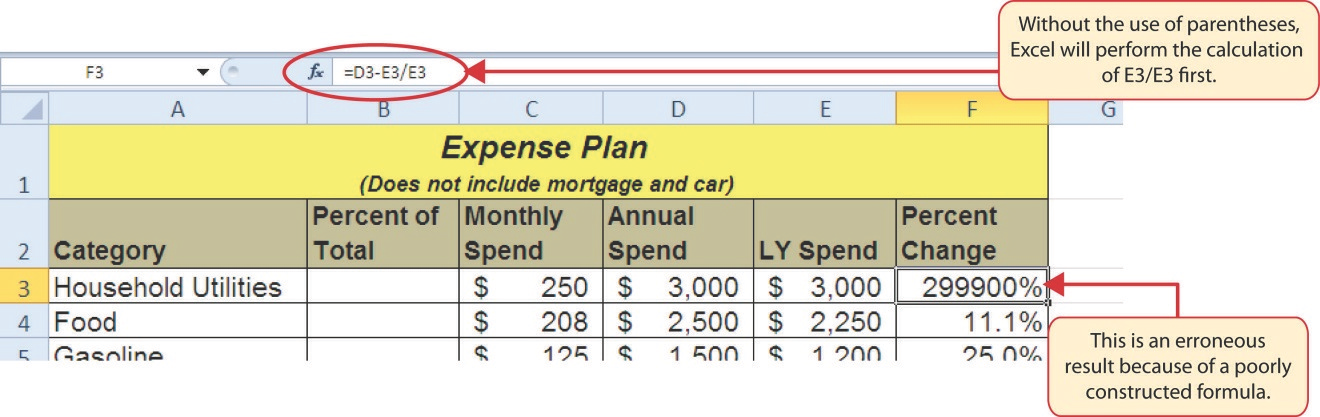
\includegraphics[width=\maxwidth{.95\linewidth}]{gfx/ch02_fig07}
	\caption{Removing the Parentheses from the Percent Change Formula}
	\label{02:fig07}
\end{figure}

\begin{center}
	\begin{sklbox}{Skill Refresher}
		\textbf{Formulas}
		\\
		\begin{itemize}
			\setlength{\itemsep}{0pt}
			\setlength{\parskip}{0pt}
			\setlength{\parsep}{0pt}
			
			\item Type an equal sign $ = $.
			\item Click or type a cell location. If using constants, type a number.
			\item Type a mathematical operator.
			\item Click or type a cell location. If using constants, type a number.
			\item Use parentheses where necessary to control the order of operations.
			\item Press the ENTER key.

			\item one
			\item two
			
		\end{itemize}
	\end{sklbox}
\end{center}

\section{Auditing Formulas}

Excel provides a few tools that you can use to review the formulas entered into a worksheet. For
example, instead of showing the outputs for the formulas used in a worksheet, you can have Excel
show the formula as it was entered in the cell locations. This is demonstrated as follows:

1. With the Budget Detail worksheet open, click the Formulas tab of the Ribbon.
2. Click the Show Formulas button in the Formula Auditing group of commands. This displays the
formulas in the worksheet instead of showing the mathematical outputs.
3. Click the Show Formulas button again. The worksheet returns to showing the output of the
formulas.

Figure 2.8 shows the Budget Detail worksheet after activating the Show Formulas command in the
Formulas tab of the Ribbon. As shown in the figure, this command allows you to view and check
all the formulas in a worksheet without having to click each cell individually. After activating this
command, the column widths in your worksheet increase significantly. The column widths were
adjusted for the worksheet shown in Figure 2.8 so all columns can be seen. The column widths return
to their previous width when the Show Formulas command is deactivated.




Integrity Check

Does the Output of Your Formula Make Sense?

It is important to note that the accuracy of the output produced by a formula depends on how it is constructed.
Therefore, always check the result of your formula to see whether it makes sense with data in your worksheet. As
shown in Figure 2.7, a poorly constructed formula can give you an inaccurate result. In other words, you can see
that there is no change between the Annual Spend and LY Spend for Household Utilities. Therefore, the result of the
%formula should be 0%. However, since the parentheses were removed in this case, the formula is clearly producing
an erroneous result.




90 NOREEN BROWN, BARBARA LAVE, JULIE ROMEY, MARY SCHATZ, DIANE SHINGLEDECKER
Figure 2.8 Show Formulas Command




Skill Refresher


Show Formulas

1. Click the Formulas tab on the Ribbon.
2. Click the Show Formulas button in the Formula Auditing group of commands.
3. Click the Show Formulas button again to show formula outputs.




Keyboard Shortcuts


Show Formulas

%• Hold down the CTRL key while pressing the accent symbol `.



Two other tools in the Formula Auditing group of commands are the Trace Precedents and Trace
Dependents commands. These commands are used to trace the cell references used in a formula. A
precedent cell is a cell whose value is used in other cells. The Trace Precedents command shows an
arrow to indicate the cells or ranges (precedents) which affect the active cell’s value. A dependent cell
is a cell whose value depends on the values of other cells in the workbook. The Trace Dependents

BEGINNING EXCEL 91
command shows where any given cell is referenced in a formula. The following is a demonstration of
these commands:

1. Click cell D3 in the Budget Detail worksheet.
2. Click the Trace Dependents button in the Formula Auditing group of commands in the
Formulas tab of the Ribbon. A double blue arrow appears, pointing to cell locations C3 and F3
(see Figure 2.9). This indicates that cell D3 is referenced in formulas that are entered in cells C3
and F3.
3. Click the Remove Arrows command in the Formula Auditing group of commands in the
Formulas tab of the Ribbon. This removes the Trace Dependents arrow.
4. Click cell F3 in the Budget Detail worksheet.
5. Click the Trace Precedents button in the Formula Auditing group of commands in the Formulas
tab of the Ribbon. A blue arrow running through cells D3 and E3 and pointing to cell F3 appears
(see Figure 2.10). This indicates that cells D3 and E3 are references in a formula entered in cell
F3.
6. Click the Remove Arrows command in the Formula Auditing group of commands in the
Formulas tab of the Ribbon. This removes the Trace Precedents arrow.
7. Save the Ch2 Personal Budget file.

Figure 2.9 shows the Trace Dependents arrow on the Budget Detail worksheet. The blue dot
represents the activated cell. The arrows indicate where the cell is referenced in formulas.




Figure 2.9 Trace Dependents Example


Figure 2.10 shows the Trace Precedents arrow on the Budget Detail worksheet. The blue dots on this
arrow indicate the cells that are referenced in the formula contained in the activated cell. The arrow
is pointing to the activated cell location that contains the formula.




92 NOREEN BROWN, BARBARA LAVE, JULIE ROMEY, MARY SCHATZ, DIANE SHINGLEDECKER
Figure 2.10 Trace Precedents Example




Skill Refresher


Trace Dependents

1. Click a cell location that contains a number or formula.
2. Click the Formulas tab on the Ribbon.
3. Click the Trace Dependents button in the Formula Auditing group of commands.
4. Use the arrow(s) to determine where the cell is referenced in formulas and functions.
5. Click the Remove Arrows button to remove the arrows from the worksheet.




Skill Refresher


Trace Precedents

1. Click a cell location that contains a formula or function.
2. Click the Formulas tab on the Ribbon.
3. Click the Trace Precedents button in the Formula Auditing group of commands.
4. Use the dot(s) along the line to determine what cells are referenced in the formula or function.
5. Click the Remove Arrows button to remove the line with the dots.




BEGINNING EXCEL 93
Key Takeaways


• Mathematical computations are conducted through formulas and functions.

• An equal sign = precedes all formulas and functions.

• Formulas and functions must be created with cell references to conduct what-if scenarios where
mathematical outputs are recalculated when one or more inputs are changed.

• Mathematical operators on a typical calculator are different from those used in Excel. Table 2.2 “Excel
Mathematical Operators” lists Excel mathematical operators.

• When using numerical values in formulas and functions, only use universal constants that do not change,
such as days in a week, months in a year, and so on.

• Relative referencing automatically adjusts the cell references in formulas and functions when they are
pasted into new locations on a worksheet. This eliminates the need to retype formulas and functions when
they are needed in multiple rows or columns on a worksheet.

• Parentheses must be used to control the order of operations when necessary for complex formulas.

• Formula auditing tools such as Trace Dependents, Trace Precedents, and Show Formulas should be used to
check the integrity of formulas that have been entered into a worksheet.



ATTRIBUTION

Adapted by Mary Schatz from How to Use Microsoft Excel: The Careers in Practice Series, adapted
by The Saylor Foundation without attribution as requested by the work’s original creator or
licensee, and licensed under CC BY-NC-SA 3.0.




94 NOREEN BROWN, BARBARA LAVE, JULIE ROMEY, MARY SCHATZ, DIANE SHINGLEDECKER
2.2 STATISTICAL FUNCTIONS




Learning Objectives


1. Use the SUM function to calculate totals.
2. Use absolute references to calculate percent of totals.
3. Use the COUNT function to count cell locations with numerical values.
4. Use the AVERAGE function to calculate the arithmetic mean.
5. Use the MAX and MIN functions to find the highest and lowest values in a range of cells.
6. Learn how to copy and paste formulas without formats applied to a cell location.
7. Learn how to set a multiple level sort sequence for data sets that have duplicate values or outputs.



In addition to formulas, another way to conduct mathematical computations in Excel is through
functions. Statistical functions apply a mathematical process to a group of cells in a worksheet. For
example, the SUM function is used to add the values contained in a range of cells. A list of commonly
used statistical functions is shown in Table 2.4. Functions are more efficient than formulas when
you are applying a mathematical process to a group of cells. If you use a formula to add the values
in a range of cells, you would have to add each cell location to the formula one at a time. This can
be very time-consuming if you have to add the values in a few hundred cell locations. However,
when you use a function, you can highlight all the cells that contain values you wish to sum in just
one step. This section demonstrates a variety of statistical functions that we will add to the Personal
Budget workbook. In addition to demonstrating functions, this section also reviews percent of total
calculations and the use of absolute references.

Table 2.4 Commonly Used Statistical Functions




BEGINNING EXCEL 95
Function     Output
ABS          The absolute value of a number
AVERAGE      The average or arithmetic mean for a group of numbers
COUNT        The number of cell locations in a range that contain a numeric character
COUNTA       The number of cell locations in a range that contain a text or numeric character
MAX          The highest numeric value in a group of numbers
The middle number in a group of numbers (half the numbers in the group are higher than the median and half the
MEDIAN
numbers in the group are lower than the median)
MIN          The lowest numeric value in a group of numbers
MODE         The number that appears most frequently in a group of numbers
PRODUCT The result of multiplying all the values in a range of cell locations
SQRT         The positive square root of a number
STDEV.S      The standard deviation for a group of numbers based on a sample
SUM          The total of all numeric values in a group


THE SUM FUNCTION

The SUM function is used when you need to calculate totals for a range of cells or a group of selected
cells on a worksheet. With regard to the Budget Detail worksheet, we will use the SUM function
to calculate the totals in row 12. It is important to note that there are several methods for adding a
function to a worksheet, which will be demonstrated throughout the remainder of this chapter. The
following illustrates how a function can be added to a worksheet by typing it into a cell location:

1.    Click the Budget Detail worksheet tab to open the worksheet.
2.    Click cell C12.
3.    Type an equal sign =.
4.    Type the function name SUM.
5.    Type an open parenthesis (.
6.    Click cell C3 and drag down to cell C11. This places the range C3:C11 into the function.
7.    Type a closing parenthesis ).
8.    Press the ENTER key. The function calculates the total for the Monthly Spend column, which is
\$1,496.

Figure 2.11 shows the appearance of the SUM function added to the Budget Detail worksheet before
pressing the ENTER key.




96 NOREEN BROWN, BARBARA LAVE, JULIE ROMEY, MARY SCHATZ, DIANE SHINGLEDECKER
Figure 2.11 Adding the SUM Function to the Budget Detail Worksheet


As shown in Figure 2.11, the SUM function was added to cell C12. However, this function is also
needed to calculate the totals in the Annual Spend and LY Spend columns. The function can be copied
and pasted into these cell locations because of relative referencing. Relative referencing serves the
same purpose for functions as it does for formulas. The following demonstrates how the total row is
completed:

1. Click cell C12 in the Budget Detail worksheet.
2. Click the Copy button in the Home tab of the Ribbon.
3. Highlight cells D12 and E12.
4. Click the Paste button in the Home tab of the Ribbon. This pastes the SUM function into cells
D12 and E12 and calculates the totals for these columns.
5. Click cell F11.
6. Click the Copy button in the Home tab of the Ribbon.
7. Click cell F12, then click the Paste button in the Home tab of the Ribbon. Since we now have
totals in row 12, we can paste the percent change formula into this row.

Figure 2.12 shows the output of the SUM function that was added to cells C12, D12, and E12. In
addition, the percent change formula was copied and pasted into cell F12. Notice that this version of
the budget is planning a 1.7% decrease in spending compared to last year.




BEGINNING EXCEL 97
Figure 2.12 Results of the SUM Function in the Budget Detail Worksheet




Integrity Check

Cell Ranges in Statistical Functions

When you intend to use a statistical function on a range of cells in a worksheet, make sure there are two cell
locations separated by a colon and not a comma. If you enter two cell locations separated by a comma, the function
will produce an output but it will be applied to only two cell locations instead of a range of cells. For example, the
SUM function shown in Figure 2.13 will add only the values in cells C3 and C11, not the range C3:C11.




98 NOREEN BROWN, BARBARA LAVE, JULIE ROMEY, MARY SCHATZ, DIANE SHINGLEDECKER
Figure 2.13 SUM Function Adding Two Cell Locations


ABSOLUTE REFERENCES (CALCULATING PERCENT OF TOTALS)

Data file: Continue with CH2 Personal Budget.

Since totals were added to row 12 of the Budget Detail worksheet, a percent of total calculation can
be added to Column B beginning in cell B3. The percent of total calculation shows the percentage
for each value in the Annual Spend column with respect to the total in cell D12. However, after the
formula is created, it will be necessary to turn off Excel’s relative referencing feature before copying
and pasting the formula to the rest of the cell locations in the column. Turning off Excel’s relative
referencing feature is accomplished through an absolute reference. The following steps explain how
this is done:

1.   Click cell B3 in the Budget Detail worksheet.
2.   Type an equal sign =.
3.   Click cell D3.
%4.   Type a forward slash /.
5.   Click cell D12.
6.   Press the ENTER key. You will see that Household Utilities represents 16.7% of the Annual
Spend budget (see Figure 2.14).




BEGINNING EXCEL 99
Figure 2.14 Adding a Formula to Calculate the Percent of Total


Figure 2.14 shows the completed formula that is calculating the percentage that Household Utilities
Annual Spend represents to the total Annual Spend for the budget (see cell B3). Normally, we would
copy this formula and paste it into the range B4:B11. However, because of relative referencing, both
cell references will increase by one row as the formula is pasted into the cells below B3. This is fine
for the first cell reference in the formula (D3) but not for the second cell reference (D12). Figure 2.15
illustrates what happens if we paste the formula into the range B4:B12 in its current state. Notice
%that Excel produces the \#DIV/0 error code. This means that Excel is trying to divide a number by
zero, which is impossible. Looking at the formula in cell B4, you see that the first cell reference was
changed from D3 to D4. This is fine because we now want to divide the Annual Spend for Insurance
by the total Annual Spend in cell D12. However, Excel has also changed the D12 cell reference to D13.
%Because cell location D13 is blank, the formula produces the \#DIV/0 error code.




100 NOREEN BROWN, BARBARA LAVE, JULIE ROMEY, MARY SCHATZ, DIANE SHINGLEDECKER
%Figure 2.15 \#DIV/0 Error from Relative Referencing


To eliminate the divide-by-zero error shown in Figure 2.15 we must add an absolute reference to
cell D12 in the formula. An absolute reference prevents relative referencing from changing a cell
reference in a formula. This is also referred to as locking a cell. The following explains how this is
accomplished:

1. Double click cell B3.
2. Place the mouse pointer in front of D12 and click. The blinking cursor should be in front of the
D in the cell reference D12.
3. Press the F4 key. You will see a dollar sign (\$) added in front of the column letter D and the row
number 12. You can also type the dollar signs in front of the column letter and row number.
4. Press the ENTER key.
5. Click cell B3.
6. Click the Copy button in the Home tab of the Ribbon.
7. Highlight the range B4:B11.
8. Click the Paste button in the Home tab of the Ribbon.

Figure 2.16 shows the percent of total formula with an absolute reference added to D12. Notice that
in cell B4, the cell reference remains D12 instead of changing to D13 as shown in Figure 2.15. Also,

BEGINNING EXCEL 101
you will see that the percentages are being calculated in the rest of the cells in the column, and the
divide-by-zero error is now eliminated.




Figure 2.16 Adding an Absolute Reference to a Cell Reference in a Formula




Skill Refresher


Absolute References

1. Click in front of the column letter of a cell reference in a formula or function that you do not want altered
when the formula or function is pasted into a new cell location.
2. Press the F4 key or type a dollar sign \$ in front of the column letter and row number of the cell reference.



THE COUNT FUNCTION

Data file: Continue with CH2 Personal Budget.

102 NOREEN BROWN, BARBARA LAVE, JULIE ROMEY, MARY SCHATZ, DIANE SHINGLEDECKER
The next function that we will add to the Budget Detail worksheet is the COUNT function. The
COUNT function is used to determine how many cells in a range contain a numeric entry. The
COUNT function will not work for counting text or other non-numeric entries. For the Budget
Detail worksheet, we will use the COUNT function to count the number of items that are planned in
the Annual Spend column (Column D). The following explains how the COUNT function is added to
the worksheet by using the function list:

1. Click cell D13 in the Budget Detail worksheet.
2. Type an equal sign =.
3. Type the letter C.
4. Click the down arrow on the scroll bar of the function list (see Figure 2.17) and find the word
COUNT.
5. Double click the word COUNT from the function list.
6. Highlight the range D3:D11.
7. You can type a closing parenthesis ) and then press the ENTER key, or simply press the ENTER
key and Excel will close the function for you. The function produces an output of 9 since there
are 9 items planned on the worksheet.

Figure 2.17 shows the function list box that appears after completing steps 2 and 3 for the COUNT
function. The function list provides an alternative method for adding a function to a worksheet.




Figure 2.17 Using the Function List to Add the COUNT Function


Figure 2.18 shows the output of the COUNT function after pressing the ENTER key. The function



BEGINNING EXCEL 103
counts the number of cells in the range D3:D11 that contain a numeric value. The result of 9 indicates
that there are 9 categories planned for this budget.




Figure 2.18 Completed COUNT Function in the Budget Detail Worksheet


THE AVERAGE FUNCTION

The next function we will add to the Budget Detail worksheet is the AVERAGE function. This
function is used to calculate the arithmetic mean for a group of numbers. For the Budget
Detail worksheet, we will use the function to calculate the average of the values in the Annual Spend
column. We will add this to the worksheet by using the Function Library. The following steps explain
how this is accomplished:

1.   Click cell D14 in the Budget Detail worksheet.
2.   Click the Formulas tab on the Ribbon.
3.   Click the More Functions button in the Function Library group of commands.
4.   Place the mouse pointer over the Statistical option from the drop-down list of options.
5.   Click the AVERAGE function name from the list of functions that appear in the menu (see
Figure 2.19). This opens the Function Arguments dialog box.
6.   Click the Collapse Dialog button in the Function Arguments dialog box (see Figure 2.20).
7.   Highlight the range D3:D11.
8.   Click the Expand Dialog button in the Function Arguments dialog box (see Figure 2.21). You can
also press the ENTER key to get the same result.
9.   Click the OK button on the Function Arguments dialog box. This adds the AVERAGE function
to the worksheet.


104 NOREEN BROWN, BARBARA LAVE, JULIE ROMEY, MARY SCHATZ, DIANE SHINGLEDECKER
Figure 2.19 illustrates how a function is selected from the Function Library in the Formulas tab of the
Ribbon.




Figure 2.19 Selecting the AVERAGE Function from the Function Library


Figure 2.20 shows the Function Arguments dialog box. This appears after a function is selected from
the Function Library. The Collapse Dialog button is used to hide the dialog box so a range of cells can
be highlighted on the worksheet and then added to the function.




Figure 2.20 Function Arguments Dialog Box


BEGINNING EXCEL 105
Figure 2.21 shows how a range of cells can be selected from the Function Arguments dialog box once
it has been collapsed.




Figure 2.21 Selecting a Range from the Function Arguments Dialog Box


Figure 2.22 shows the Function Arguments dialog box after the cell range is defined for the
AVERAGE function. The dialog box shows the result of the function before it is added to the cell
location. This allows you to assess the function output to determine whether it makes sense before
adding it to the worksheet.




106 NOREEN BROWN, BARBARA LAVE, JULIE ROMEY, MARY SCHATZ, DIANE SHINGLEDECKER
Figure 2.22 Function Arguments Dialog Box after a Cell Range Is Defined for a Function


Figure 2.23 shows the completed AVERAGE function in the Budget Detail worksheet. The output
of the function shows that on average we expect to spend \$1,994 for each of the categories listed in
Column A of the budget. This average spend calculation per category can be used as an indicator to
determine which categories are costing more or less than the average budgeted spend dollars.




Figure 2.23 Completed AVERAGE Function


THE MAX AND MIN FUNCTIONS

Data file: Continue with CH2 Personal Budget.

BEGINNING EXCEL 107
The final two statistical functions that we will add to the Budget Detail worksheet are the MAX
and MIN functions. These functions identify the highest and lowest values in a range of cells. The
following steps explain how to add these functions to the Budget Detail worksheet:

1.   Click cell D15 in the Budget Detail worksheet.
2.   Type an equal sign =.
3.   Type the word MIN.
4.   Type an open parenthesis (.
5.   Highlight the range D3:D11.
6.   Type a closing parenthesis ) and press the ENTER key, or simply press the ENTER key and
Excel will close the function for you. The MIN function produces an output of $1,200, which is
the lowest value in the Annual Spend column (see Figure 2.24).
7.   Click cell D16.
8.   Type an equal sign =.
9.   Type the word MAX.
10.   Type an open parenthesis (.
11.   Highlight the range D3:D11.
12.   Type a closing parenthesis ) and press the ENTER key, or simply press the ENTER key and
Excel will close the function for you. The MAX function produces an output of $3,500. This is
the highest value in the Annual Spend column (see Figure 2.25).




Figure 2.24 MIN Function Added to the Budget Detail Worksheet




108 NOREEN BROWN, BARBARA LAVE, JULIE ROMEY, MARY SCHATZ, DIANE SHINGLEDECKER
Figure 2.25 MAX Function Added to the Budget Detail Worksheet




Skill Refresher


Statistical Functions

1. Type an equal sign =.
2. Type the function name followed by an open parenthesis ( or double click the function name from the
function list.
3. Highlight a range on a worksheet or click individual cell locations followed by commas.
4. Type a closing parenthesis ) and press the ENTER key or press the ENTER key to close the function.



COPY AND PASTE FORMULAS (PASTING WITHOUT FORMATS)

Data file: Continue with CH2 Personal Budget.

As shown in Figure 2.25, the COUNT, AVERAGE, MIN, and MAX functions are summarizing the
data in the Annual Spend column. You will also notice that there is space to copy and paste these
functions under the LY Spend column. This allows us to compare what we spent last year and what we
are planning to spend this year. Normally, we would simply copy and paste these functions into the
range E13:E16. However, you may have noticed the double-line style border that was used around the
perimeter of the range B13:E16. If we used the regular Paste command, the double line on the right
side of the range E13:E16 would be replaced with a single line. Therefore, we are going to use one

BEGINNING EXCEL 109
of the Paste Special commands to paste only the functions without any of the formatting treatments.
This is accomplished through the following steps:

1.    Highlight the range D13:D16 in the Budget Detail worksheet.
2.    Click the Copy button in the Home tab of the Ribbon.
3.    Click cell E13.
4.    Click the down arrow below the Paste button in the Home tab of the Ribbon.
5.    Click the Formulas option from the drop-down list of buttons (see Figure 2.26).

Figure 2.26 shows the list of buttons that appear when you click the down arrow below the Paste
button in the Home tab of the Ribbon. One thing to note about these options is that you can preview
them before you make a selection by dragging the mouse pointer over the options. As shown in the
figure, when the mouse pointer is placed over the Formulas button, you can see how the functions
will appear before making a selection. Notice that the double-line border does not change when this
option is previewed. That is why this selection is made instead of the regular Paste option.




Figure 2.26 Paste Formulas Option




Skill Refresher


Paste Formulas



110 NOREEN BROWN, BARBARA LAVE, JULIE ROMEY, MARY SCHATZ, DIANE SHINGLEDECKER
1. Click a cell location containing a formula or function.
2. Click the Copy button in the Home tab of the Ribbon.
3. Click the cell location or cell range where the formula or function will be pasted.
4. Click the down arrow below the Paste button in the Home tab of the Ribbon.
5. Click the Formulas button under the Paste group of buttons.



SORTING DATA (MULTIPLE LEVELS)

Data file: Continue with CH2 Personal Budget.

The Budget Detail worksheet shown in Figure 2.26 is now producing several mathematical outputs
through formulas and functions. The outputs allow you to analyze the details and identify trends as
to how money is being budgeted and spent. Before we draw some conclusions from this worksheet,
we will sort the data based on the Percent of Total column. Sorting is a powerful tool that enables you
to analyze key trends in any data set. Sorting will be covered thoroughly in a later chapter, but will
be briefly introduced here. For the purposes of the Budget Detail worksheet, we want to set multiple
levels for the sort order. This is accomplished through the following steps:

1. Highlight the range A2:F11 in the Budget Detail worksheet.
2. Click the Data tab in the Ribbon.
3. Click the Sort button in the Sort \& Filter group of commands. This opens the Sort dialog box, as
shown in Figure 2.27.
4. Click the down arrow next to the “Sort by” box.
5. Click the Percent of Total option from the drop-down list.
6. Click the down arrow next to the sort Order box.
7. Click the Largest to Smallest option.
8. Click the Add Level button. This allows you to set a second level for any duplicate values in the
Percent of Total column.
9. Click the down arrow next to the “Then by” box.
10. Select the LY Spend option. Leave the Sort Order as Smallest to Largest
11. Click the OK button at the bottom of the Sort dialog box.
12. Save the Ch2 Personal Budget file.




BEGINNING EXCEL 111
Figure 2.27 Sort Dialog Box


Figure 2.28 shows the Budget Detail worksheet after it has been sorted. Notice that there are three
identical values in the Percent of Total column. This is why a second sort level had to be created for
this worksheet. The second sort level arranges the values of 8.4% based on the values in the LY Spend
column in ascending order. Excel gives you the option to set as many sort levels as necessary for the
data contained in a worksheet.




112 NOREEN BROWN, BARBARA LAVE, JULIE ROMEY, MARY SCHATZ, DIANE SHINGLEDECKER
Figure 2.28 Budget Detail Worksheet after Sorting




Skill Refresher


Sorting Data (Multiple Levels)

1. Highlight a range of cells to be sorted.
2. Click the Data tab of the Ribbon.
3. Click the Sort button in the Sort \& Filter group.
4. Select a column from the “Sort by” drop-down list in the Sort dialog box.
5. Select a sort order from the Order drop-down list in the Sort dialog box.
6. Click the Add Level button in the Sort dialog box.
7. Repeat Steps 4 and 5.
8. Click the OK button on the Sort dialog box.



Now that the Budget Detail worksheet is sorted, a few key trends can be easily identified. The
BEGINNING EXCEL 113
worksheet clearly shows that the top three categories as a percentage of total budgeted spending for
the year are Taxes, Household Utilities, and Food. All three categories are necessities (or realities) of
life and typically require a significant amount of income for most households. Looking at the Percent
Change column, we can see how our planned spending is expected to change from last year. This is
perhaps the most important column on the worksheet because it allows you to assess whether your
plan is realistic. You will see that there are no changes planned for Taxes and Household Utilities.
While Taxes can change from year to year, it is not too difficult to predict what they will be. In this
case, we are assuming that there are no changes to the tax costs for our budget. We are also planning
no change in Household Utilities. These costs can fluctuate from year to year as well. However, you
can take measures to reduce costs, such as using less electricity, turning off heat when no one is in the
house, keeping track of your wireless minutes so you do not go over the maximum allowed in your
plan, and so on. As a result, there is no change in planned spending for Household Utilities because
we will assume that any rate increases will be offset with a decrease in usage. The third item that is
planned not to change is Insurance. Insurance policies for cars and homes can change, but as is true
for taxes, the changes are predictable. Therefore, we are assuming no changes in our insurance policy.

The first big change that is noticeable in the worksheet is the Food and Entertainment categories in
rows 5 and 6 (see definitions in Table 2.1). The Percent Change column indicates that there is an 11.1%
decrease in Entertainment spending and an 11.1% increase in Food spending. This is logical because
if you plan to eat in restaurants less frequently, you will be eating at home more frequently. Although
this makes sense in theory, it may be hard to do in practice. Dinners and parties with friends may be
tough to turn down. However, the entire process of maintaining a budget is based on discipline, and
it certainly takes a significant amount of discipline to plan targets for yourself and stick to them.

A few other points to note are the changes in the Gasoline and Vacation categories. If you commute
to school or work, the price of gas can have a significant impact on your budget. It is important
to be realistic if gas prices are increasing, and you should reflect these increases in your budget. To
compensate for the increased spending for gas, the spending plan for vacations has been reduced by
25%. Budgeting often requires a certain degree of creativity. Although the Vacation budget has been
reduced, there is still money you can set aside to make plans for spring break or winter break.

Finally, the budget shows a decrease in Miscellaneous spending of 19.8%. This was defined as a group
containing several expenses, such as textbooks, school supplies, software updates, and so on (see
Table 2.1). You may be able to reduce your spending in this category if you can use items such as
online textbooks. This reduction in spending can free up funds for Clothes, a spend category that has
increased by 20%. We will continue to develop the Personal Budget workbook further in Section 2.3
“Functions for Personal Finance”.


Key Takeaways


• Statistical functions are used when a mathematical process is required for a range of cells, such as summing
the values in several cell locations. For these computations, functions are preferable to formulas because
adding many cell locations one at a time to a formula can be very time-consuming.



114 NOREEN BROWN, BARBARA LAVE, JULIE ROMEY, MARY SCHATZ, DIANE SHINGLEDECKER
• Statistical functions can be created using cell ranges or selected cell locations separated by commas. Make
sure you use a cell range (two cell locations separated by a colon) when applying a statistical function to a
contiguous range of cells.

• To prevent Excel from changing the cell references in a formula or function when they are pasted to a new
cell location, you must use an absolute reference. You can do this by placing a dollar sign (\$) in front of the
column letter and row number of a cell reference.

• The \#DIV/0 error appears if you create a formula that attempts to divide a constant or the value in a cell
reference by zero.

• The Paste Formulas option is used when you need to paste formulas without any formatting treatments into
cell locations that have already been formatted.

• You need to set multiple levels, or columns, in the Sort dialog box when sorting data that contains several
duplicate values.



ATTRIBUTION

Adapted by Mary Schatz from How to Use Microsoft Excel: The Careers in Practice Series, adapted
by The Saylor Foundation without attribution as requested by the work’s original creator or
licensee, and licensed under CC BY-NC-SA 3.0.




BEGINNING EXCEL 115
2.3 FUNCTIONS FOR PERSONAL FINANCE




Learning Objectives


1. Understand the fundamentals of loans and leases.
2. Use the PMT function to calculate monthly mortgage payments on a house.
3. Use the PMT function to calculate monthly lease payments for an automobile.
4. Learn how to summarize data in a workbook by using worksheet links to create a summary worksheet.



In this section, we continue to develop the Personal Budget workbook. Notable items that are
missing from the Budget Detail worksheet are the payments you might make for a car or a home.
This section demonstrates Excel functions used to calculate lease payments for a car and to calculate
mortgage payments for a house.

THE FUNDAMENTALS OF LOANS AND LEASES

One of the functions we will add to the Personal Budget workbook is the PMT function. This function
calculates the payments required for a loan or a lease. However, before demonstrating this function,
it is important to cover a few fundamental concepts on loans and leases.

A loan is a contractual agreement in which money is borrowed from a lender and paid back over
a specific period of time. The amount of money that is borrowed from the lender is called
the principal of the loan. The borrower is usually required to pay the principal of the loan plus
interest. When you borrow money to buy a house, the loan is referred to as a mortgage. This is because
the house being purchased also serves as collateral to ensure payment. In other words, the bank can
take possession of your house if you fail to make loan payments. As shown in Table 2.5, there are
several key terms related to loans and leases.

Table 2.5 Key Terms for Loans and Leases




116 NOREEN BROWN, BARBARA LAVE, JULIE ROMEY, MARY SCHATZ, DIANE SHINGLEDECKER
Term        Definition
Collateral Any item of value that is used to secure a loan to ensure payments to the lender
Down        The amount of cash paid toward the purchase of a house. If you are paying 20% down, you are paying 20% of the cost
Payment     of the house in cash and are borrowing the rest from a lender.
Interest
The interest that is charged to the borrower as a cost for borrowing money
Rate
Mortgage A loan where property is put up for collateral
Principal   The amount of money that has been borrowed
Residual
The estimated selling price of a vehicle at a future point in time
Value
Terms       The amount of time you have to repay a loan


Figure 2.29 shows an example of an amortization table for a loan. A lender is required by law to
provide borrowers with an amortization table when a loan contract is offered. The table in the figure
shows how the payments of a loan would work if you borrowed $100,000 from a lender and agreed to
pay it back over 10 years at an interest rate of 5%. You will notice that each time you make a payment,
you are paying the bank an interest fee plus some of the loan principal. Each year the amount of
interest paid to the bank decreases and the amount of money used to pay off the principal increases.
This is because the bank is charging you interest on the amount of principal that has not been paid. As
you pay off the principal, the interest rate is applied to a lower number, which reduces your interest
charges. Finally, the figure shows that the sum of the values in the Interest Payment column is $29,505.
This is how much it costs you to borrow this money over 10 years. Indeed, borrowing money is not
free. It is important to note that to simplify this example, the payments were calculated on an annual
basis. However, most loan payments are made on a monthly basis.




BEGINNING EXCEL 117
Figure 2.29 Example of an Amortization Table


A lease is a contract in which you, the lessee, use an asset such as a car or a piece of equipment and you
agree to make regular payments to the owner or the lessor. When you lease a car, the manufacturer
or a leasing company retains ownership of the vehicle and you agree to make regular payments for a
specific period of time. The amount of money you pay depends on the price of the car, the terms of
the lease contract, and the car’s expected residual value at the end of the lease. The calculation of lease
payments is similar to the calculation of loan payments. However, when you lease a car, you pay only
the value of the car that is used. For example, suppose you are leasing a car that is priced at $25,000.
The lease contract is for 4 years at an interest rate of 5%. The residual value of the car is $10,000. This
means the car will lose $15,000 of its value over 4 years. Another way to state this is that the car will
depreciate $15,000. A lease will be structured so that you pay this $15,000 in depreciation. However,

118 NOREEN BROWN, BARBARA LAVE, JULIE ROMEY, MARY SCHATZ, DIANE SHINGLEDECKER
the interest charges will be based on the purchase price of \$25,000. We will look at a demonstration
of leasing a car as well as buying a home in the next section.

THE PMT (PAYMENT) FUNCTION FOR LOANS

Data file: Continue with CH2 Personal Budget.

If you own a home, your mortgage payments are a major component of your household budget. If you
are planning to buy a home, having a clear understanding of your monthly payments is critical for
maintaining strong financial health. In Excel, mortgage payments are conveniently calculated through
the PMT (payment) function. This function is more complex than the statistical functions covered in
Section 2.2 “Statistical Functions”. With statistical functions, you are required to add only a range of
cells or selected cells within the parentheses of the function, also known as the argument. With the
PMT function, you must accurately define a series of arguments in order for the function to produce
a reliable output. Table 2.6 lists the arguments for the PMT function. It is helpful to review the key
loan and lease terms in Table 2.5 before reviewing the PMT function arguments.

Table 2.6 Arguments for the PMT Function

Argument Definition
This is the interest rate the lender is charging the borrower. The interest rate is usually quoted in annual terms, so
Rate
you have to divide this rate by 12 if you are calculating monthly payments.
The argument letters stand for number of periods. This is the term of the loan, which is the amount of time you have
Nper      to repay the bank. This is usually quoted in years, so you have to multiply the years by 12 if you are calculating
monthly payments.
The argument letters stand for present value. This is the principal of the loan or the amount of money that is
Pv        borrowed. When defining this argument, a minus sign must precede the cell location or value. For leases, this
argument is used for the price of the item being leased.
The argument letters stand for future value. The brackets around the argument indicate that it is not always
[Fv]      necessary to define it. It is used if there is a lump-sum payment that will be made at the end of the loan terms. This is
also used for the residual value of a lease. If it is not defined, Excel will assume that it is zero.
This argument can be defined with either a 1 or a 0. The number 1 is used if payments are made at the beginning of
each period. A 0 is used if payments are made at the end of each period. The argument is in brackets because it does
[Type]
not have to be defined if payments are made at the end of each period. Excel assumes that this argument is 0 if it is
not defined.


By default, the result of the PMT function in Excel is shown as a negative number. This is because
it represents an outgoing payment. When making a mortgage or car payment, you are paying money
out of your pocket or bank account. Depending on the type of work that you do, your employer may
want you to leave your payments negative or they may ask you to format them as positive numbers.
In the following assignments, the payments calculated using the PMT function will be made positive
to make them easier to work with. To do this, when defining the PV argument (amount of money
borrowed) in the PMT dialog box, a minus sign must precede the cell location or value (see the PV
argument in Figure 2.32).

We will use the PMT function in the Personal Budget workbook to calculate the monthly mortgage
payments for a house. These calculations will be made in the Mortgage Payments worksheet and
then displayed in the Budget Summary worksheet through a cell reference link. So far we have
demonstrated several methods for adding functions to a worksheet. The following steps explain a new
method using the Insert Function command for adding the PMT function:
BEGINNING EXCEL 119
1.   Click the Mortgage Payments worksheet tab.
2.   Click cell B5.
3.   Click the Formulas tab on the Ribbon.
4.   Click the Insert Function button (see Figure 2.30). This opens the Insert Function dialog box,
which can be used for searching all functions in Excel.
5.   In the “Search for a function:” input box at the top of the Insert Function dialog box,
type mortgage payments (see Figure 2.31). Note that the current description in the “Search for
a function:” input box will already be highlighted. You can begin typing and the description will
be replaced with your entry.
6.   Click the Go button in the upper right side of the Insert Function dialog box. This adds all the
Excel functions that match your description in the “Select a function:” box in the lower half of
the Insert Function dialog box (see Figure 2.31).
7.   Click the PMT option in the “Select a function:” box in the lower half of the Insert Function
dialog box.
8.   Click the OK button at the lower right side of the Insert Function dialog box. This will open the
Function Arguments dialog box.




120 NOREEN BROWN, BARBARA LAVE, JULIE ROMEY, MARY SCHATZ, DIANE SHINGLEDECKER
Figure 2.30 Mortgage Payments Worksheet




BEGINNING EXCEL 121
Figure 2.31 Insert Function Dialog Box




9. Click the Collapse Dialog button next to the Rate argument in the Function Arguments dialog
box. This will be the first argument defined for the function (see Figure 2.32)
10. Click cell B3 on the worksheet. This is the rate being charged on the loan.
11. Type a forward slash / for division.
12. Type the number 12. Since our goal is to calculate the monthly payments for the loan, we need
to divide the rate, which is stated in annual terms, by 12. This converts the annual rate to a
monthly rate.
13. Press the ENTER key on your keyboard. This returns the Function Arguments dialog box to its
expanded form. You will also see that the Rate argument is now defined.
14. Click the Collapse Dialog button next to the Nper argument in the Function Arguments dialog
box. This is the second argument we define in the function.
15. Click cell B4 on the worksheet. This is the term or the amount of time we have to repay the loan.
16. Type an asterisk * for multiplication.
17. Type the number 12. Since our goal is to calculate the monthly payments for the loan, we need
to multiply the terms of the loan by 12. This converts the terms of the loan from years to
months.
18. Press the ENTER key on your keyboard. This returns the Function Arguments dialog box to its
expanded form. You will also see that the Nper argument is now defined.
19. Click the Collapse Dialog button next to the Pv argument in the Function Arguments dialog
box. This is the third argument we will define in the function.
20. Type a minus sign -. When defining the Pv argument of the PMT function, any cell location or
value must be preceded with a minus sign.
21. Click cell B2 on the worksheet. This is the principal of the loan.
122 NOREEN BROWN, BARBARA LAVE, JULIE ROMEY, MARY SCHATZ, DIANE SHINGLEDECKER
22. Press the ENTER key on your keyboard. You will now see the Rate, Nper, and Pv arguments
defined for the function.
23. Click the OK button at the bottom of the Function Arguments dialog box. The function will
now be placed into the worksheet. Since we are not paying any lump sums of money at the end
of the loan, there is no need to define the Fv argument. Also, we will assume that the monthly
mortgage payments will be made at the end of each month. Therefore, there is no need to define
the Type argument.


Keyboard Shortcuts


Insert Function

• Hold the SHIFT key while pressing the F3 key.

Function Arguments Dialog Box

• After the equal sign = and function name are typed into cell a location, hold down the CTRL key and press
the letter A on your keyboard.



Figure 2.32 shows the completed Function Arguments dialog box for the PMT function. Notice that
the dialog box shows the values for the Rate and Nper arguments. The Rate is divided by 12 to convert
the annual interest rate to a monthly interest rate. The Nper argument is multiplied by 12 to convert
the terms of the loan from years to months. Finally, the dialog box provides you with a definition for
each argument. The definition appears when you click in the input box for the argument.




Figure 2.32 Function Arguments Dialog Box for the PMT Function




BEGINNING EXCEL 123
Figure 2.33 shows the final appearance of the Mortgage Payments worksheet after the PMT function
is added. The result of the function in cell B5 will be displayed in the Budget Summary worksheet.




Figure 2.33 Mortgage Payments Worksheet with the PMT Function




Integrity Check

Comparable Arguments for PMT Function

When using functions such as PMT, make sure the arguments are defined in comparable terms. For example, if you
are calculating the monthly payments of a loan, make sure both the Rate and Nper argument are expressed in terms
of months. The function will produce an erroneous result if one argument is expressed in years while the other is
expressed in months.




124 NOREEN BROWN, BARBARA LAVE, JULIE ROMEY, MARY SCHATZ, DIANE SHINGLEDECKER
THE PMT (PAYMENT) FUNCTION FOR LEASES

In addition to calculating the mortgage payments for a home, the PMT function will be used in the
Personal Budget workbook to calculate the lease payments for a car. The details for the lease payments
are found in the Car Lease Payments worksheet. Similar to the statistical functions, we can either
type the PMT function directly into a cell or use the Insert Function button. However, you must know
the definitions for each argument of the function and understand how these arguments need to be
defined based on your objective. The terms for loans and leases are in Table 2.5, and the definitions
for the arguments of the PMT function are in Table 2.6. The following steps explain how the PMT
function is added to the Personal Budget workbook to calculate the lease payments for a car:

1. Click cell B6 in the Car Lease Payments worksheet.
2. Click the Formulas tab on the Ribbon.
3. Click the Financial button in the Function Library group. This opens the Financial Function
drop down list.
4. Scroll down and click on the PMT Function in the drop down list. This will open the PMT
Function Arguments dialog box. See Figure 2.34.
5. Click the Collapse Dialog button next to the Rate argument in the PMT Function Arguments
dialog box. This will be the first argument defined for the monthly car lease payment.
6. Click cell B4. This is the interest rate being charged for the lease.
7. Type the forward slash / for division.
8. Type the number 12. Since our goal is to calculate the monthly lease payments, we divide the
interest rate by 12 to convert the annual rate to a monthly rate.
9. Press the ENTER key on your keyboard. This returns the Function Arguments dialog box to its
expanded form. You will also see that the Rate argument is now defined.
10. Click the Collapse Dialog button next to the Nper argument in the Function Arguments dialog
box. This is the second argument we define in the function.
11. Click cell B5. This is the term or the length of time for the lease contract. Since the term is
already expressed in months, we can just reference cell B5 and move to the next argument. If the
term was defined in years, instead of months, we would need to multiply the terms (years) of the
loan by 12 to convert the years to months.
12. Press the ENTER key on your keyboard. This returns the Function Arguments dialog box to its
expanded form. You will also see that the Nper argument is now defined.
13. Click the Collapse Dialog button next to the Pv argument in the Function Arguments dialog
box. This is the third argument we will define in the function.
14. Type a minus sign -. Remember that cell locations or values used to define the Pv argument
must be preceded with a minus sign.
15. Click cell B2 on the worksheet, which is the price of the car.
16. Press the ENTER key on your keyboard. You will now see the Rate, Nper, and Pv arguments
defined for the function.
17. Click the Collapse Dialog button next to the Fv argument in the Function Arguments dialog
box. This is the fourth argument we will define in the function.
18. Click cell B3 on the worksheet. This is the residual value of the car. Note that cell location and
values used to define the [Fv] argument are NOT preceded by a minus sign.


BEGINNING EXCEL 125
19. Press the ENTER key on your keyboard. You will now see the Rate, Nper, Pv and Fv arguments
defined for the function.
20. Click the Collapse Dialog button next to the Type argument in the Function Arguments dialog
box. This is the fifth and last argument we will define in the function.
21. Type the number 1. We will assume that the lease payments will be due at the beginning of each
month. For payments made at the beginning of the period, a 1 will be entered in the Type
argument box. For payments made at the end of the period, a 0 will be entered in the Type
argument box.
22. Press the ENTER key. You will now see the Rate, Nper, Pv, Fv and Type arguments defined for
the function. See Figure 2.34.
23. Click the OK button at the bottom of the Function Arguments dialog box. The function will
now be placed into the worksheet.

Figure 2.34 shows how the the completed Function Arguments dialog box for the PMT function car
lease should appear before pressing the OK button.




Figure 2-34 Function Arguments Dialog Box for the PMT Lease Function


Figure 2.35 shows the result of the PMT function for the car lease. The monthly payments for this
lease are \$206.56. This monthly payment will be displayed in the Budget Summary worksheet.




126 NOREEN BROWN, BARBARA LAVE, JULIE ROMEY, MARY SCHATZ, DIANE SHINGLEDECKER
Figure 2.35 Results of the PMT Function in the Car Lease Payments Worksheet




Skill Refresher


PMT Function

1. Type an equal sign =.
2. Type the letters PMT followed by an open parenthesis, or double click the function name from the
function list.
3. Define the Rate argument with a cell location that contains the rate being charged by the lender for the
loan or lease. If the interest rate given is an annual rate, divide it by 12 to convert it to a monthly rate.
4. Define the Nper argument with a cell location that contains the amount of time to repay the loan or lease.
If the amount of time is in years, multiply it by 12 to convert it to number of months.
5. Define the Pv argument with a cell location that contains the principal of the loan or the price of the item
being leased. Cell locations or values used for this argument must be preceded by a minus sign.
6. Define the [Fv] argument with a cell location that contains the residual value of the item being leased or
the lump sum payment for a loan.
7. Define the [Type] argument with a 1 if payments are made at the beginning of each period or 0 if payments
are made at the end of each period.



BEGINNING EXCEL 127
8. Type a closing parenthesis ).
9. Press the ENTER key.



LINKING WORKSHEETS (CREATING A SUMMARY WORKSHEET)

So far we have used cell references in formulas and functions, which allow Excel to produce new
outputs when the values in the cell references are changed. Cell references can also be used to display
values or the outputs of formulas and functions in cell locations on other worksheets. This is how data
will be displayed on the Budget Summary worksheet in the Personal Budget workbook. Outputs
from the formulas and functions that were entered into the Budget Detail, Mortgage Payments,
and Car Lease Payments worksheets will be displayed on the Budget Summary worksheet through
the use of cell references. The following steps explain how this is accomplished:

1.   Click cell C3 in the Budget Summary worksheet.
2.   Type an equal sign =.
3.   Click the Budget Detail worksheet tab.
4.   Click cell D12 on the Budget Detail worksheet.
5.   Press the ENTER key on your keyboard. The output of the SUM function in cell D12 on
the Budget Detail worksheet will be displayed in cell C3 on the Budget Summary worksheet.

Figure 2.36 shows how the cell reference appears in the Budget Summary worksheet. Notice that
the cell reference D12 is preceded by the Budget Detail worksheet name enclosed in apostrophes
followed by an exclamation point (‘Budget Detail’!) This indicates that the value displayed in the cell
is referencing a cell location in the Budget Detail worksheet.




128 NOREEN BROWN, BARBARA LAVE, JULIE ROMEY, MARY SCHATZ, DIANE SHINGLEDECKER
Figure 2.36 Cell Reference Showing the Total Expenses in the Budget Summary Worksheet


As shown in Figure 2.36, the Budget Summary worksheet is designed to show the expense budget
for the mortgage payments and the auto lease payments. However, you will recall that we used the
PMT function to calculate the monthly payments. In the Budget Summary worksheet, we need to
show the total annual payments. As a result, we will create a formula that references cell locations in
the Mortgage Payments and Car Lease Payments worksheets. The following steps explain how this
is accomplished:

1.   Click cell C4 in the Budget Summary worksheet.
2.   Type an equal sign =.
3.   Click the Mortgage Payments worksheet tab.
4.   Click cell B5 in the Mortgage Payments worksheet.
5.   Type an asterisk * for multiplication.
6.   Type the number 12. This multiplies the monthly payments by 12 to calculate the total payments
required for the year. The formula in the formula bar should read: =’Mortgage Payments’!B5*12
7.   Press the ENTER key on your keyboard. The value of multiplying the monthly mortgage
payments by 12 is now displayed on the Budget Summary worksheet.
8.   Click cell C5 on the Budget Summary worksheet.
9.   Type an equal sign =.
10.   Click the Car Lease Payments worksheet tab.
11.   Click cell B6 in the Car Lease Payments worksheet.
12.   Type an asterisk * for multiplication.
13.   Type the number 12. This multiplies the monthly lease payments by 12 to calculate the total
payments required for the year.
14.   Press the ENTER key on your keyboard. The value of multiplying the monthly lease payments
by 12 is now displayed on the Budget Summary worksheet.
BEGINNING EXCEL 129
Figure 2.37 shows the results of creating formulas that reference cell locations in the Mortgage
Payments and Car Lease Payments worksheets.




Figure 2.37 Formulas Referencing Cells in Mortgage Payments and Car Lease Payments Worksheets


We can now add other formulas and functions to the Budget Summary worksheet that can calculate
the difference between the total spend dollars vs. the total net income in cell D2. The following steps
explain how this is accomplished:

1.   Click cell D6 in the Budget Summary worksheet.
2.   Type an equal sign =.
3.   Type the function name SUM followed by an open parenthesis (.
4.   Highlight the range C3:C5.
5.   Type a closing parenthesis ) and press the ENTER key on your keyboard or simply press the
ENTER key to close the function. The total for all annual expenses now appears on the
worksheet.
6.   Click cell D7 on the Budget Summary worksheet. You will enter a formula to calculate Net
Change in Cash in this cell.
7.   Type an equal sign =.
8.   Click cell D2.
9.   Type a minus sign - and then click cell D6.
10.   Press the ENTER key on your keyboard. This formula produces an output of \$1,942, indicating
our income is greater than our total expenses.

Figure 2.38 shows the results of the formulas that were added to the Budget Summary worksheet.
The output for the formula in cell D7 shows that the net income exceeds total planned expenses by
130 NOREEN BROWN, BARBARA LAVE, JULIE ROMEY, MARY SCHATZ, DIANE SHINGLEDECKER
\$1,942. Overall, having your income exceed your total expenses is a good thing because it allows you
to save money for future spending needs or unexpected events.




Figure 2.38 Formulas Added to Show Income Is Greater Than Expenses


We can now add a few formulas that calculate both the spending rate and the savings rate as a
percentage of net income. These formulas require the use of absolute references, which we covered
earlier in this chapter. The following steps explain how to add these formulas:

1.   Click cell E6 in the Budget Summary worksheet.
2.   Type an equal sign =.
3.   Click cell D6.
4.   Type a forward slash / for division and then click D2.
5.   Press the F4 key on your keyboard. This adds an absolute reference to cell D2.
6.   Press the ENTER key. The result of the formula shows that total expenses consume 94.1% of our
net income.
7.   Click cell E6.
8.   Place the mouse pointer over the Auto Fill Handle.
9.   When the mouse pointer turns to a black plus sign, left click and drag down to cell E7. This
copies and pastes the formula into cell E7.
10.   Save the CH2 Personal Budget file.
11.   Compare your work with the self-check answer key (found in the Course Files link) and then
submit the CH2 Personal Budget workbook as directed by your instructor.
12.   Close the CH2 Personal Budget file before moving on to 2.4 – Preparing to Print.

Figure 2.39 shows the output of the formulas calculating the spending rate and savings rate as a
BEGINNING EXCEL 131
percentage of net income. The absolute reference shown for cell D2 prevents the cell from changing
when the formula is copied from cell E6 and pasted into cell E7. The results of the formula show that
our current budget allows for a savings rate of 5.9%. This is a fairly good savings rate.




Figure 2.39 Calculating the Savings Rate




Key Takeaways


• The PMT function can be used to calculate the monthly mortgage payments for a house or the monthly lease
payments for a car.

• When using the PMT function, each argument must be separated by a comma.

• To calculate the monthly payment for a loan using the PMT function, the Rate and Nper arguments must be
defined in terms of months. The Rate should be divided by 12 to convert it from an annual rate to a monthly
rate. The Nper should be multiplied by 12 to convert the term of the loan from years to months.

• The PMT function produces a negative output if the Pv argument is not preceded by a minus sign. For the
purposes of this textbook, a minus sign will be entered before the PV argument in the PMT dialog box.



ATTRIBUTION

Adapted by Mary Schatz from How to Use Microsoft Excel: The Careers in Practice Series, adapted
by The Saylor Foundation without attribution as requested by the work’s original creator or
licensee, and licensed under CC BY-NC-SA 3.0.

132 NOREEN BROWN, BARBARA LAVE, JULIE ROMEY, MARY SCHATZ, DIANE SHINGLEDECKER
2.4 PREPARING TO PRINT




Learning Objectives


1. Review and learn new cell formatting techniques.
2. Understand how to modify page scaling and margins.
3. Create custom headers and footers to automatically update information.



In this section, we will review some of the formatting techniques covered in Chapter 1, as well as
learn some new techniques. We will also preview a two-page worksheet and set page setup options to
present the data in a professional manner. A new data file will be used in this section.




BEGINNING EXCEL 133
Figure 2.40 Finished Prepare to Print Worksheet in Print Preview


134 NOREEN BROWN, BARBARA LAVE, JULIE ROMEY, MARY SCHATZ, DIANE SHINGLEDECKER
FORMATTING WORKSHEET DATA

Download Data File: CH2 PTP Data

You have been given sales data that needs to be formatted in a professional manner. This worksheet
will be printed and presented to investors, so it needs to be prepared for printing as well. Figure 2.40
shows how the finished worksheet will appear in Print Preview.

1. Open the Data file named CH2 PTP Data and use the File/Save As command to save it with the
new name CH2 Sales Data.
2. To change the font of the entire worksheet, click the Select All button in the top left corner of
the worksheet grid (see Figure 2.41).




Figure 2.41 Select All button


3. Change the font to Calibri, Size 12.
4. Using the skills learned in Chapter 1, make the following formatting changes:

1. A1:H1 – Merge and Center; format text as bold and apply a font color and size of your
choice
2. A2:H2 – Merge and Center; format text as bold and italic, apply a font color of your choice
3. A5:H5 – Apply a dark fill color; format text as white and bold
4. C5:H5 – Center align
5. A15:H15 – Apply Top Border to the cells; format text as bold
6. C6:H6 and C15:H15 – Apply Accounting Number format with 0 decimal places
7. C7:H14 – Apply Comma style with 0 decimal places
8. Highlight A6:A14 (salespeople’s names) and click the Increase Indent button in the
Alignment group on the Home ribbon (see Figure 2.42). This will indent the text from the
cell border.




Figure 2.42 Increase Indent button




BEGINNING EXCEL 135
USING PAGE SETUP OPTIONS

Once the worksheet is professionally formatted, you need to look in Print Preview to see how the
pages will print.

1. With the CH2 Sales Data file still open, go to Backstage View by clicking the File tab on the
ribbon. Select Print from the menu. Notice that the worksheet is currently printing on two
pages, with the page breaking between the April and May columns. To fix this problem, you will
first change the left and right margins while still in Print Preview
2. Click the Margins drop-down arrow in the Settings section (see Figure 2.43)
3. Select Custom Margins… at the bottom of the list.
4. Type in 0.5 for the Left Margin and 0.5 for the Right Margin.
5. Click OK. Changing the margins brought the May column onto the same page, but the June
column is still on a separate page. Next you will use Page Scaling to fix this while still in Print
Preview.
6. Click the Scaling drop-down arrow in the Settings section (Figure 2.43).
7. Select Fit All Columns on One Page.
8. Exit Backstage View.




Figure 2.43 Settings section of Print Preview


CREATING A FOOTER USING PAGE SETUP

Now that the entire worksheet is printing on one page, you need to add a footer with information
136 NOREEN BROWN, BARBARA LAVE, JULIE ROMEY, MARY SCHATZ, DIANE SHINGLEDECKER
about the date the file was printed along with the filename. In Chapter 1 you learned how to create
headers and footers using the Insert ribbon. You can also create headers and footers using the Custom
Header/Footer dialog box.

1. Click the Page Layout tab on the ribbon.
2. Click the dialog box launcher in the Page Setup group. A window similar to Figure 2.44 should
appear.




Figure 2.44 Page Setup Dialog Box


3. Click the Header/Footer tab in the Page Setup dialog box.
4. Click the Custom Footer button. The Footer dialog box should appear (see Figure 2.45).




BEGINNING EXCEL 137
Figure 2.45 Footer Dialog Box


5.   Click in the Left section: box and type Printed on.
6.   Making sure to leave a space after the word on, click the Insert Date button.
7.   Click in the Right section: box and type Filename:.
8.   Making sure to leave a space after the colon, click the Insert File Name button.
9.   The Footer dialog box should look like Figure 2.46.
10.   Click the OK button. Click OK again to close the Page Setup dialog box.
11.   Go to Print Preview to see that the current date and file name are displayed in the footer.
12.   Exit Backstage View. Save the CH2 Sales Data file.
13.   Compare your work with the self-check answer key (found in the Course Files link) and then
submit the CH2 Sales Data workbook as directed by your instructor.




Figure 2.46 Completed Custom Footer Dialog Box




Key Takeaways


• It is important to always check your workbooks in Print Preview to ensure that the data is printed in a
professional and easy to read manner.

• Adjust margins and page scaling as needed to keep columns of data together on one page if possible.



138 NOREEN BROWN, BARBARA LAVE, JULIE ROMEY, MARY SCHATZ, DIANE SHINGLEDECKER
• Use headers and footers to display information in the top and bottom margins of the printed worksheet.
Use the Insert buttons to insert changing information, such as dates and file names, instead of typing them
in directly.



ATTRIBUTION

“2.4 Preparing to Print” by Julie Romey, Portland Community College is licensed under CC BY 4.0




BEGINNING EXCEL 139
2.5 CHAPTER PRACTICE




FINANCIAL PLAN FOR A LAWN CARE BUSINESS

Download Data File: PR2 Data

Running your own lawn care business can be an excellent way to make money over the summer while
on break from college. It can also be a way to supplement your existing income for the purpose of
saving money for retirement or for a college fund. However, managing the costs of the business will
be critical in order for it to be a profitable venture. In this exercise you will create a simple financial
plan for a lawn care business by using the skills covered in this chapter.

1. Open the file named PR2 Data and then Save As PR2 Lawn Care.
2. Click cell C5 in the Annual Plan worksheet.
3. Write a formula that calculates the average price per lawn cut. Do not use the AVERAGE
function. The formula should be the Price per Acre multiplied by the Average Acreage per
Customer.
4. Click cell C8.
5. Enter a formula that calculates the total number of lawns that will be cut during the year
(Number of Customers * Frequency of Lawn Cuts per Customer).
6. Click cell D9.
7. Enter a formula that calculates the total sales for the plan (Average Price per Cut * Total Lawn
Cuts).
8. Click cell F3 in the Leases worksheet. The PMT function will be used to calculate the monthly
lease payment for the first item. For many businesses, leasing (or renting) equipment is a more
favorable option than purchasing equipment because it requires far less cash. This enables you
to begin a business such as a lawn care business without having to put up a lot of money to buy
equipment. The PMT function can be entered using the Insert Function button as seen in
Chapter 2, or we can type the PMT function directly into a cell. For this assignment, we will
type the function into cell F3 using the following instructions.
9. Type =PMT(. Define the arguments of the function as follows:
10. Rate: Click cell B3, type a forward slash / for division, type the number 12, and type a comma ,.
Since we are calculating monthly payments, the annual interest rate must be converted to a
monthly interest rate by dividing by 12.
11. Nper: Click cell C3, type *12 and then type a comma ,. Similar to the Rate argument, the terms
of the lease must be converted to months by multiplying by 12 since we are calculating monthly
payments.


140 NOREEN BROWN, BARBARA LAVE, JULIE ROMEY, MARY SCHATZ, DIANE SHINGLEDECKER
12. Pv: Type a minus sign -, click cell D3, and type a comma ,. Remember that this argument must
always be preceded by a minus sign.
13. Fv: Click cell E3 (Residual Value) and type a comma ,.
14. Type: Type the number 1, type a closing parenthesis ), and press the ENTER key. We will assume
the lease payments will be made at the beginning of each month, which requires that this
argument be defined with a value of 1.
15. Copy the PMT function in cell F3 and paste it into the range F4:F6, or use the Autofill handle.
16. Click cell F10 in the Leases worksheet. Enter an Autosum function to calculate the total for the
monthly lease payments. Make sure that blank rows (7 through 9) were included in the range for
the SUM function. If other items are added to the worksheet, they will be included in the output
of the SUM function.
17. Highlight the range A2:F6 on the Leases worksheet. The data in this range will be sorted, first by
Interest Rate and then by Price. Click the Sort button in the Data tab of the Ribbon. In the Sort
dialog box, select the Interest Rate option in the “Sort by” drop-down box. Select Largest to
Smallest for the sort order. Then, click the Add Level button on the Sort dialog box. Select the
Price option in the “Then by” drop-down box. Select Largest to Smallest for the sort order. Click
the OK button in the Sort dialog box.
18. Click cell B11 on the Annual Plan worksheet. The monthly lease payments that are calculated
in the Lease worksheet will be displayed in this cell.
19. Type an equal sign =. Click the Leases worksheet, click cell F10, and press the ENTER key.
20. Click cell C12 on the Annual Plan worksheet. Create a formula that calculates the annual lease
payments. This should be the Monthly Lease Payments * 12.
21. Click cell C14 on the Annual Plan worksheet. Create a formula that calculates the Total Lawn \&
Equipment Expenses (Lawn \& Equipment Expenses per Cut * Total Lawn Cuts).
22. Click cell D16 on the Annual Plan worksheet. Enter a SUM function that adds the Expenses for
the business in column C. Make sure to add the Expenses only (not the Sales Plan information).
23. Click cell D17 on the Annual Plan worksheet. Enter a formula that calculates the annual profit
(Operating Income) for the business. This should be the Total Sales – Total Expenses.
24. Format all cells that contain money amounts in the Annual Plan worksheet for Accounting
Number Format (\$) with no decimals.
25. Click cell B10 on the Investments worksheet. Enter a COUNT function that counts the number
of investments that currently have a balance in column B. Make sure that the additional blank
rows in rows 6 through 8 are included in the range for this function. The function output will
automatically change if any new investments are added to the worksheet. It is important to note,
however, that the Total in cell B9 should not be included in the Count range.
26. Click cell D3 on the Investments worksheet.
27. Type an equal sign =. Click the Annual Plan worksheet. Click cell D17 and type a forward slash
/ for division. Click the Investments worksheet. Click cell B10 and press the ENTER key. This
formula divides the profit calculated on the Annual Plan worksheet by the number of
investments in the Investments worksheet. We will assume that the profits from this business
will be invested evenly among the funds listed in Column A of the Investments worksheet.
28. Before copying and pasting the formula created in cell D3, absolute references must be added to
the cell locations in the formula. Edit the formula in cell D3 on the Investments worksheet so
that cells D17 and B10 are absolute. The formula in cell D3 should be: ='Annual Plan'!$D$17/

BEGINNING EXCEL 141
Investments!$B$10. When you copy the formula in cell D3 down, the cell references will not
change, because they are absolute. The formula will continue to divide the Operating Income in
cell D17 of the Annual Plan by the Number of Investments in cell B10 of the Investments sheet.
29.   Copy cell D3 and paste it into cells D4 and D5 or use the Auto Fill handle to copy down.
30.   Click cell B9 on the Investments worksheet. Enter a SUM function that adds the current balance
for all investments in column B. Make sure that blank rows (rows 6 through 8) are added to the
range for the function so additional investments will automatically be included in the Autosum
function output.
31.   Copy the SUM function in cell B9 and paste it into cell D9.
32.   Format the Investments and Leases sheets appropriately for Accounting Format. This should
include $ signs on the top row and total row for money amounts, and comma style in the middle
rows. In the Investments sheet, apply Comma Style with 0 decimals to the ranges B4:B5 and
D4:D5. In the Leases worksheet, apply Accounting Number Format ($) with two decimals to the
range D3:F3 and F10. Apply comma format with two decimals to the range D4:F9. Double check
that your formatting matches Figures 2.47a through 2.47c.
33.   Save the PR2 Lawn Care workbook.
34.   Compare your work with the self-check answer key (found in the Course Files link) and then
submit the PR2 Lawn Care workbook as directed by your instructor.




Figure 2.47a Completed Lawn Care Annual Plan Worksheet


142 NOREEN BROWN, BARBARA LAVE, JULIE ROMEY, MARY SCHATZ, DIANE SHINGLEDECKER
Figure 2.47b Completed Lawn Care Investments Worksheet




BEGINNING EXCEL 143
Figure 2.47c Completed Lawn Care Leases Worksheet


ATTRIBUTION

Adapted by Mary Schatz from How to Use Microsoft Excel: The Careers in Practice Series, adapted
by The Saylor Foundation without attribution as requested by the work’s original creator or
licensee, and licensed under CC BY-NC-SA 3.0.




144 NOREEN BROWN, BARBARA LAVE, JULIE ROMEY, MARY SCHATZ, DIANE SHINGLEDECKER
2.6 CHAPTER SCORED




HOTEL OCCUPANCY AND EXPENSES

Download Data File: SC2 Data

The hotel management industry presents a wide variety of career opportunities. These range from
running a bed and breakfast to a management position at a large hotel. No matter what hotel
management career you choose to pursue, understanding hotel occupancy and costs are critical to
running a successful operation. This exercise examines the occupancy rate and expenses of a small
hotel.

1. Open the file named SC2 Data and then Save As SC2 Hotel.
2. Enter a formula in cell C5 on the Occupancy worksheet to calculate the January capacity for
the hotel. The capacity shows how many people the hotel can hold during the month. It is
calculated by first multiplying the occupants per room by the number of rooms in the hotel.
This result is then multiplied by the number of days in the month (cell B5 for January). Create
this formula using absolute references so that the appropriate cells do not change when the
formula is pasted throughout column C. Hint: two of the cells in the formula need to be absolute
references.
3. Copy the formula in cell C5 and paste it into the range C6:C16. Use a paste method that does
not remove the border at the bottom of cell C16.
4. Enter a formula in cell E5 on the Occupancy worksheet to calculate the Percent Occupied of
the hotel (this statistic shows what percentage of the hotel is full or occupied). Your formula
should divide the Actual Occupancy by the Hotel Capacity. Then copy and paste the formula
into the range E6:E16. Use a paste method that does not remove the border at the bottom of cell
E16. Format the results in E5:E16 as percentages with two decimal places.
5. Enter a function in cell C17 on the Occupancy worksheet that sums the values in the range
C5:C16. Copy the function and paste it into cell D17.
6. Copy the formula in cell E16 and paste it into cell E17. Make sure cell E17 is formatted as a
percentage with two decimals and bold.
7. On the Statistics worksheet, enter a function into cell B3 that shows the highest value (Max) in
the range D5:D16 in the Actual Occupancy column on the Occupancy worksheet.
8. On the Statistics worksheet, enter a function into cell B4 that shows the lowest value (Min) in
the range D5:D16 in the Actual Occupancy column on the Occupancy worksheet.
9. On the Statistics worksheet, enter a function into cell B5 that shows the average value in the
range D5:D16 in the Actual Occupancy column on the Occupancy worksheet.
10. Use the Auto Fill handle to copy the formulas in the range B3:B5 to the range C3:C5.
BEGINNING EXCEL 145
11. Format the range B3:B5 for comma format with zero decimal places. Format cells C3:C5 as
percentages with two decimal places.
12. The hotel is considering buying or leasing a car to shuttle customers to and from the airport.
You hope to keep the monthly payment under \$400 and will determine whether leasing or
buying will meet that goal. On the Lease or Buy worksheet, type the terms in Figure 2.48 below
for the purchase vs. lease of the car. Make sure that dollar amounts and percentages are
formatted to match Figure 2.48:




Figure 2.48 Terms for the purchase vs. lease of the car


13. In cell B8 create a PMT function to calculate the Monthly Payment if you purchase the car.
Make sure the arguments in the PMT function are converted into months and that the Monthly
Payment is a positive number.
14. In cell C8 create a PMT function to calculate the Monthly Payment if you lease the car. The car
will have a residual value of \$15,000 when the lease is over. Assume that payments are made at
the end of the month.
15. Format the Monthly Payments in B8:C8 for Accounting Number Format with two decimals.
16. Select the range A4:A8 and click the Increase Indent button once to indent the labels in column
A.
17. From the Page Layout tab, access the Page Setup dialog box launcher and center the Lease or
Buy worksheet horizontally on the page.
18. Insert a footer on the Lease or Buy worksheet. Insert the date (use the Insert Date button) in the
left section of the footer. Insert the File Name (use the Insert File Name button) in the right
section of the footer.
19. Save the SC2 Hotel workbook.
20. Submit the SC2 Hotel workbook as directed by your instructor.

ATTRIBUTION

Adapted by Mary Schatz from How to Use Microsoft Excel: The Careers in Practice Series, adapted
by The Saylor Foundation without attribution as requested by the work’s original creator or
licensee, and licensed under CC BY-NC-SA 3.0.

